% =============================================================================
% Tricopter LQR Flight Controller — Full Technical Report
% =============================================================================
\documentclass[12pt, a4paper]{article}

% --- Packages ---
\usepackage[utf8]{inputenc}
\usepackage[T1]{fontenc}
\usepackage{amsmath, amssymb, amsfonts}
\usepackage{bm}                % bold math symbols
\usepackage{geometry}
\geometry{margin=2.5cm}
\usepackage{graphicx}
\usepackage{booktabs}
\usepackage{enumitem}
\usepackage{hyperref}
\hypersetup{colorlinks=true, linkcolor=blue, citecolor=blue, urlcolor=blue}
\usepackage{listings}
\usepackage{xcolor}
\usepackage{float}
\usepackage{caption}
\usepackage{subcaption}
\usepackage{tikz}
\usetikzlibrary{arrows.meta, positioning, shapes.geometric, calc}

% Code listing style
\lstdefinestyle{cppstyle}{
    language=C++,
    basicstyle=\ttfamily\footnotesize,
    keywordstyle=\color{blue}\bfseries,
    commentstyle=\color{gray}\itshape,
    stringstyle=\color{red},
    numbers=left,
    numberstyle=\tiny\color{gray},
    stepnumber=1,
    numbersep=5pt,
    breaklines=true,
    frame=single,
    backgroundcolor=\color{gray!5},
    tabsize=4,
    showstringspaces=false,
    captionpos=b,
}
\lstdefinestyle{yamlstyle}{
    basicstyle=\ttfamily\footnotesize,
    commentstyle=\color{gray}\itshape,
    numbers=left,
    numberstyle=\tiny\color{gray},
    breaklines=true,
    frame=single,
    backgroundcolor=\color{gray!5},
    tabsize=2,
    showstringspaces=false,
    captionpos=b,
}
\lstset{style=cppstyle}

% Shorthand commands
\newcommand{\R}{\mathbb{R}}
\newcommand{\bx}{\bm{x}}
\newcommand{\bu}{\bm{u}}
\newcommand{\bq}{\bm{q}}
\newcommand{\bomega}{\bm{\omega}}
\newcommand{\btau}{\bm{\tau}}
\newcommand{\bF}{\bm{F}}
\newcommand{\bJ}{\bm{J}}
\newcommand{\bK}{\bm{K}}
\newcommand{\bA}{\bm{A}}
\newcommand{\bB}{\bm{B}}
\newcommand{\bP}{\bm{P}}
\newcommand{\bQ}{\bm{Q}}
\newcommand{\bR}{\bm{R}}
\newcommand{\bI}{\bm{I}}
\newcommand{\bzero}{\bm{0}}

\title{%
    \textbf{Cascaded Flight Controller for a Servoless Asymmetric Tricopter} \\[6pt]
    \large Inner-Loop Attitude LQR + Outer-Loop Altitude PID \\[4pt]
    \large Complete Mathematical Derivation, Software Architecture, \\ and Implementation Guide
}
\author{Auto-generated Technical Report}
\date{\today}

\begin{document}
\maketitle
\tableofcontents
\newpage

% =============================================================================
\section{Introduction and Motivation}
% =============================================================================

\subsection{What Is a Tricopter?}

A \textbf{tricopter} is a type of multirotor aircraft that uses exactly three propellers (rotors) to fly.  Each propeller is driven by a brushless DC motor.  Compared with the more common quadcopter (four rotors), a tricopter has one fewer actuator.  This makes it mechanically simpler but significantly harder to control.

In a quadcopter the four motors are typically arranged symmetrically and alternate in spin direction (clockwise / counter-clockwise), so the reaction torques cancel perfectly at equal speed.  With only three rotors, the reaction torques \emph{cannot} cancel in general, and a traditional tricopter uses a \textbf{yaw servo} --- a small motor that tilts the rear propeller --- to generate the missing yaw torque.

Our vehicle is a \textbf{servoless} tricopter: it has no yaw servo.  Yaw control must come entirely from the \emph{differential reaction torques} of the three fixed-spin propellers.  Furthermore, the rotor positions are \textbf{asymmetric} (the triangle formed by the three rotors is \emph{not} equilateral), and the full $3\times3$ inertia tensor has off-diagonal coupling terms.

\subsection{Why a Cascaded Controller?}

A ``full-state'' LQR on all 12 states (position, velocity, attitude, angular rate) was tried previously and proved unstable.  The reason is that the translational and rotational dynamics operate on very different time scales and magnitudes.  A single LQR mixes them, leading to poorly conditioned gain matrices.

Instead we use a \textbf{cascaded} architecture:
\begin{enumerate}[label=\arabic*.]
    \item \textbf{Inner loop (fast):} an attitude-only LQR that stabilises roll, pitch, and yaw using a 6-state linearised model.
    \item \textbf{Outer loop (slow):} a simple PID controller that regulates altitude by commanding total thrust.
\end{enumerate}
The inner loop runs ``inside'' the outer loop: the altitude PID adjusts collective thrust, while the attitude LQR adjusts differential motor speeds.

\subsection{Control Input Parameterisation}

A critical design choice: we use $\omega_i^2$ (the \emph{square} of each motor's angular velocity) as the control variable, \textbf{not} thrust directly.  Why?  Because both the thrust force and the reaction drag torque of a propeller are \emph{linear} in $\omega^2$:
\begin{align}
    T_i &= k_{T,i} \, \omega_i^2  \label{eq:thrust} \\
    Q_i &= k_{Q,i} \, \omega_i^2  \label{eq:drag}
\end{align}
where $k_T$ is the thrust coefficient and $k_Q$ is the drag torque coefficient of the propeller.  Because both are linear in $\omega^2$, the mapping from the control vector $\bu = [\omega_1^2, \omega_2^2, \omega_3^2]^T$ to forces and torques is a \emph{linear matrix equation}, which is exactly what LQR requires.

% =============================================================================
\section{Vehicle Model}
% =============================================================================

\subsection{Coordinate Frames}

We use two coordinate frames:
\begin{itemize}
    \item \textbf{World frame} (inertial): $x$ forward, $y$ left, $z$ up.  Gravity points in the $-z$ direction: $\bm{g} = [0, 0, -9.81]^T$ m/s$^2$.
    \item \textbf{Body frame}: fixed to the vehicle's centre of gravity (CG).  Axes align with the vehicle's principal directions.  All rotor positions, thrust axes, and spin axes are specified in this frame.
\end{itemize}

\subsection{Rotor Configuration}

Each rotor $i$ (where $i = 1, 2, 3$) is described by:
\begin{itemize}
    \item $\bm{r}_i \in \R^3$: position vector from the CG to the rotor, in body frame [m].
    \item $\hat{\bm{t}}_i \in \R^3$: unit thrust axis (direction of thrust force).
    \item $\hat{\bm{s}}_i \in \R^3$: unit spin axis (axis about which the propeller rotates).
    \item $d_i \in \{+1, -1\}$: spin direction ($+1$ = clockwise, $-1$ = counter-clockwise when viewed from above).
    \item $k_{T,i}$: thrust coefficient [N$\cdot$s$^2$/rad$^2$].
    \item $k_{Q,i}$: drag torque coefficient [N$\cdot$m$\cdot$s$^2$/rad$^2$].
\end{itemize}

For our default configuration:
\begin{table}[H]
\centering
\begin{tabular}{lccccc}
\toprule
\textbf{Rotor} & \textbf{Position} [m] & $\hat{\bm{t}}_i$ & $d_i$ & $k_T$ & $k_Q$ \\
\midrule
0 (front)       & $(0.25, 0, 0)$       & $(0,0,1)$ & $+1$ & $1.5\times10^{-5}$ & $2.5\times10^{-7}$ \\
1 (rear-left)   & $(-0.15, 0.20, 0)$   & $(0,0,1)$ & $-1$ & $1.5\times10^{-5}$ & $2.5\times10^{-7}$ \\
2 (rear-right)  & $(-0.15, -0.20, 0)$  & $(0,0,1)$ & $+1$ & $1.5\times10^{-5}$ & $2.5\times10^{-7}$ \\
\bottomrule
\end{tabular}
\caption{Default rotor configuration.  Note the asymmetric positions and two CW vs one CCW spin direction.}
\label{tab:rotors}
\end{table}

\subsection{Inertia Tensor}

The vehicle has mass $m = 1.5$ kg and a \emph{full} (non-diagonal) inertia tensor:
\begin{equation}
    \bJ = \begin{bmatrix} J_{xx} & J_{xy} & J_{xz} \\ J_{xy} & J_{yy} & J_{yz} \\ J_{xz} & J_{yz} & J_{zz} \end{bmatrix}
    = \begin{bmatrix} 0.03 & 0.001 & 0.0005 \\ 0.001 & 0.025 & 0.0008 \\ 0.0005 & 0.0008 & 0.04 \end{bmatrix}
    \; \text{kg}\cdot\text{m}^2
\end{equation}
The off-diagonal terms arise because the vehicle is not symmetric about any axis.  A diagonal inertia tensor would imply perfect symmetry.

% =============================================================================
\section{Control Allocation}
\label{sec:control_alloc}
% =============================================================================

\subsection{The Allocation Matrix $\bB_{\text{alloc}}$}

The \textbf{control allocation matrix} is the linear map from motor commands $\bu = [\omega_1^2, \omega_2^2, \omega_3^2]^T$ to the total body-frame forces and torques:
\begin{equation}
    \begin{bmatrix} \bF_{\text{body}} \\ \btau_{\text{body}} \end{bmatrix}
    = \bB_{\text{alloc}} \, \bu
    \qquad
    \bB_{\text{alloc}} \in \R^{6 \times 3}
\end{equation}

Each column of $\bB_{\text{alloc}}$ represents the force and torque produced by rotor $i$ per unit $\omega_i^2$.

\subsubsection{Force Column}

The force from rotor $i$ is simply thrust along its thrust axis:
\begin{equation}
    \bm{f}_i = k_{T,i} \, \hat{\bm{t}}_i
\end{equation}
For our rotors with $\hat{\bm{t}}_i = [0, 0, 1]^T$ and $k_T = 1.5 \times 10^{-5}$, every force column is $[0, 0, 1.5 \times 10^{-5}]^T$.

\subsubsection{Torque Column}

The torque from rotor $i$ has \textbf{two components}:

\paragraph{1. Moment from thrust (cross-product torque).}  The thrust force $\bm{f}_i$ acts at position $\bm{r}_i$ from the CG, creating a moment:
\begin{equation}
    \btau_{\text{thrust},i} = \bm{r}_i \times (k_{T,i} \, \hat{\bm{t}}_i)
\end{equation}
This is the familiar ``force times lever arm'' torque.  For example, a rotor offset in the $y$-direction creates a roll torque (about the $x$-axis).

\paragraph{2. Reaction (drag) torque.}  As the propeller spins, aerodynamic drag on the blades produces a torque that opposes the rotation.  By Newton's third law, this reaction torque is applied to the vehicle:
\begin{equation}
    \btau_{\text{drag},i} = d_i \, k_{Q,i} \, \hat{\bm{s}}_i
\end{equation}
The sign $d_i = \pm 1$ indicates the spin direction.  A clockwise-spinning propeller ($d_i = +1$) creates a positive torque about the spin axis on the vehicle body.

\paragraph{Total torque column:}
\begin{equation}
    \btau_i = \bm{r}_i \times (k_{T,i} \, \hat{\bm{t}}_i) + d_i \, k_{Q,i} \, \hat{\bm{s}}_i
    \label{eq:torque_col}
\end{equation}

\subsubsection{Worked Example: Rotor 0 (Front)}

\begin{align}
    \bm{f}_0 &= 1.5 \times 10^{-5} \cdot [0, 0, 1]^T = [0, 0, 1.5 \times 10^{-5}]^T \\
    \btau_{\text{thrust},0} &= [0.25, 0, 0]^T \times [0, 0, 1.5 \times 10^{-5}]^T \\
    &= \begin{bmatrix}
        0 \cdot 1.5\times10^{-5} - 0 \cdot 0 \\
        0 \cdot 0 - 0.25 \cdot 1.5\times10^{-5} \\
        0.25 \cdot 0 - 0 \cdot 0
    \end{bmatrix}
    = \begin{bmatrix} 0 \\ -3.75 \times 10^{-6} \\ 0 \end{bmatrix} \\
    \btau_{\text{drag},0} &= (+1) \cdot 2.5 \times 10^{-7} \cdot [0, 0, 1]^T = [0, 0, 2.5 \times 10^{-7}]^T \\
    \btau_0 &= [0, \; -3.75 \times 10^{-6}, \; 2.5 \times 10^{-7}]^T
\end{align}

The front rotor creates \emph{negative} pitch torque (nose-down tendency due to its forward position) and a small positive yaw torque (reaction from CW spin).

\subsection{The Full Allocation Matrix}

Assembling all columns:
\begin{equation}
    \bB_{\text{alloc}} = \begin{bmatrix}
        0 & 0 & 0 \\
        0 & 0 & 0 \\
        1.5\times10^{-5} & 1.5\times10^{-5} & 1.5\times10^{-5} \\
        0 & 3.0\times10^{-6} & -3.0\times10^{-6} \\
        -3.75\times10^{-6} & 2.25\times10^{-6} & 2.25\times10^{-6} \\
        2.5\times10^{-7} & -2.5\times10^{-7} & 2.5\times10^{-7}
    \end{bmatrix}
\end{equation}
Rows 1--3 are force ($\bB_{\text{force}}$), rows 4--6 are torque ($\bB_\tau$).

\subsection{Controllability Analysis of $\bB_\tau$}

The torque sub-block $\bB_\tau \in \R^{3 \times 3}$ tells us how well we can control the three torque axes (roll, pitch, yaw):
\begin{equation}
    \bB_\tau = \begin{bmatrix}
        0 & 3.0\times10^{-6} & -3.0\times10^{-6} \\
        -3.75\times10^{-6} & 2.25\times10^{-6} & 2.25\times10^{-6} \\
        2.5\times10^{-7} & -2.5\times10^{-7} & 2.5\times10^{-7}
    \end{bmatrix}
\end{equation}

The \textbf{singular value decomposition} (SVD) reveals:
\begin{align}
    \sigma_1 &= 4.92 \times 10^{-6} \quad \text{(strongest axis)} \\
    \sigma_2 &= 4.26 \times 10^{-6} \\
    \sigma_3 &= 1.61 \times 10^{-7} \quad \text{(weakest axis --- yaw)}
\end{align}

The \textbf{condition number} $\kappa = \sigma_1 / \sigma_3 = 30.6$.  This means the yaw axis is about 30 times weaker than the strongest torque axis.  The \textbf{rank} is 3 (full rank), meaning all three torque axes \emph{are} controllable, but yaw has very limited authority.

\subsection{Physical Interpretation}

Roll and pitch are controlled by the large lever arms of the rotor positions (up to $\bm{r}_i = 0.25$ m), multiplied by $k_T = 1.5 \times 10^{-5}$, giving torque sensitivity $\sim 3.75 \times 10^{-6}$ N$\cdot$m per unit $\omega^2$.

Yaw is controlled \emph{only} by the tiny drag torque coefficient $k_Q = 2.5 \times 10^{-7}$, which is about 15 times smaller.  This weak yaw authority is a fundamental property of servoless tricopters.

% =============================================================================
\section{Hover Trim}
\label{sec:trim}
% =============================================================================

\subsection{The Trim Problem}

``Trim'' means finding the motor speeds that produce \textbf{steady hover}: the vehicle hangs motionless in the air.  This requires:
\begin{enumerate}
    \item \textbf{Force balance:} Total thrust equals weight.
    \begin{equation}
        \sum_{i=1}^{3} k_{T,i} \, (\hat{\bm{t}}_i \cdot \hat{\bm{z}}) \, u_i = m g
        \label{eq:thrust_balance}
    \end{equation}
    where $u_i = \omega_i^2$ and $\hat{\bm{z}} = [0,0,1]^T$.

    \item \textbf{Torque balance:} Net torque is zero.
    \begin{equation}
        \bB_\tau \, \bu = \bm{0}
        \label{eq:torque_balance}
    \end{equation}
\end{enumerate}

\subsection{Why Exact Trim Is Impossible}

Equation~\eqref{eq:torque_balance} is 3 equations in 3 unknowns.  Equation~\eqref{eq:thrust_balance} adds a 4th equation.  Together we have \textbf{4 equations in 3 unknowns} --- an \emph{overdetermined} system.

Since $\bB_\tau$ is full rank (rank 3), the only solution to $\bB_\tau \bu = \bm{0}$ is $\bu = \bm{0}$, which gives zero thrust.  Therefore, \textbf{no motor speed combination can simultaneously produce zero torque and nonzero thrust} for this vehicle geometry.

This is a fundamental consequence of having 3 actuators and 4 constraints.  Conventional tricopters solve this with a yaw servo (4th actuator).

\subsection{The KKT Optimisation}

Since we cannot satisfy all 4 constraints exactly, we find the \emph{best compromise}: minimise the residual torque while exactly meeting the thrust requirement.  This is a \textbf{constrained quadratic optimisation}:
\begin{equation}
    \min_{\bu} \; \bu^T \underbrace{\bB_\tau^T \bB_\tau}_{\bm{M}} \bu
    \qquad \text{subject to} \quad \bm{c}^T \bu = mg
\end{equation}
where $\bm{c} = [k_{T,1}, k_{T,2}, k_{T,3}]^T$ is the thrust coefficient vector (assuming $\hat{\bm{t}}_i \cdot \hat{\bm{z}} = 1$).

The \textbf{Karush-Kuhn-Tucker (KKT)} conditions for this problem are obtained by forming the Lagrangian:
\begin{equation}
    \mathcal{L}(\bu, \lambda) = \bu^T \bm{M} \bu + \lambda \, (\bm{c}^T \bu - mg)
\end{equation}
Setting $\nabla_{\bu} \mathcal{L} = 0$ and $\nabla_\lambda \mathcal{L} = 0$:
\begin{equation}
    \begin{bmatrix} 2\bm{M} & \bm{c} \\ \bm{c}^T & 0 \end{bmatrix}
    \begin{bmatrix} \bu \\ \lambda \end{bmatrix}
    = \begin{bmatrix} \bm{0} \\ mg \end{bmatrix}
    \label{eq:kkt}
\end{equation}
This is a $(N{+}1) \times (N{+}1)$ linear system (4$\times$4 for our tricopter) that we solve directly.

\subsection{Trim Results}

The KKT solver produces:
\begin{align}
    \omega_0^2 &= 367{,}242 \quad \Rightarrow \quad \omega_0 = 606.0 \;\text{rad/s} \quad \text{(front)} \\
    \omega_1^2 &= 308{,}145 \quad \Rightarrow \quad \omega_1 = 555.1 \;\text{rad/s} \quad \text{(rear-left)} \\
    \omega_2^2 &= 305{,}613 \quad \Rightarrow \quad \omega_2 = 552.8 \;\text{rad/s} \quad \text{(rear-right)}
\end{align}
The speeds are \textbf{unequal}, as expected.  The front rotor spins fastest because:
\begin{itemize}
    \item It must produce the most thrust for pitch balance (its lever arm is largest: $x = 0.25$ m vs $0.15$ m for the rear pair).
    \item Being the sole CW rotor at the front, it carries extra yaw-balancing burden.
\end{itemize}

The residual torque is $[0.0076, \; 0.0038, \; 0.0912]^T$ Nm, with most of the residual in yaw (0.091 Nm).  This is the unavoidable physical limitation discussed above.

% =============================================================================
\section{Rigid Body Dynamics}
\label{sec:dynamics}
% =============================================================================

\subsection{State Vector}

The full nonlinear state vector has 13 components:
\begin{equation}
    \bx = \begin{bmatrix}
        p_x \\ p_y \\ p_z \\ v_x \\ v_y \\ v_z \\ q_w \\ q_x \\ q_y \\ q_z \\ \omega_x \\ \omega_y \\ \omega_z
    \end{bmatrix}
    \in \R^{13}
\end{equation}
where:
\begin{itemize}
    \item $\bm{p} = [p_x, p_y, p_z]^T$: position in world frame [m].
    \item $\bm{v} = [v_x, v_y, v_z]^T$: velocity in world frame [m/s].
    \item $\bq = [q_w, q_x, q_y, q_z]^T$: unit quaternion representing body-to-world rotation.
    \item $\bomega = [\omega_x, \omega_y, \omega_z]^T$: angular velocity in body frame [rad/s].
\end{itemize}

\subsection{Why Quaternions?}

We represent attitude using \textbf{quaternions} rather than Euler angles because:
\begin{enumerate}
    \item \textbf{No gimbal lock.}  Euler angles have a singularity at $\pm 90°$ pitch where yaw and roll become indistinguishable.  Quaternions are singularity-free.
    \item \textbf{Smooth integration.}  Quaternion kinematics are a simple linear ODE in $\bomega$, making numerical integration stable.
    \item \textbf{Efficient rotation.}  Converting a quaternion to a rotation matrix requires only 9 multiplications and 6 additions.
\end{enumerate}

A unit quaternion $\bq = [q_w, q_x, q_y, q_z]^T$ with $\|\bq\| = 1$ represents a rotation.  The scalar part $q_w$ encodes the half-angle of rotation, and the vector part $[q_x, q_y, q_z]$ encodes the axis.

The rotation matrix from body to world frame is:
\begin{equation}
    \bm{R}(\bq) = \begin{bmatrix}
        1 - 2(q_y^2 + q_z^2) & 2(q_x q_y - q_w q_z) & 2(q_x q_z + q_w q_y) \\
        2(q_x q_y + q_w q_z) & 1 - 2(q_x^2 + q_z^2) & 2(q_y q_z - q_w q_x) \\
        2(q_x q_z - q_w q_y) & 2(q_y q_z + q_w q_x) & 1 - 2(q_x^2 + q_y^2)
    \end{bmatrix}
\end{equation}

\subsection{Translational Dynamics}

Newton's second law in the world frame:
\begin{equation}
    m \, \dot{\bm{v}} = \bm{R}(\bq) \, \bF_{\text{body}} + m \, \bm{g}
    \label{eq:trans_dyn}
\end{equation}
where $\bF_{\text{body}} = \bB_{\text{force}} \, \bu$ is the total force in the body frame and $\bm{g} = [0, 0, -9.81]^T$ m/s$^2$.

The rotation matrix $\bm{R}(\bq)$ transforms the body-frame force into the world frame.  At hover ($\bq = [1,0,0,0]$, i.e.\ identity rotation), $\bm{R} = \bI$ and the thrust points straight up.  When the vehicle tilts, $\bm{R}$ redirects some thrust sideways.

\subsection{Rotational Dynamics (Euler's Equation)}

The angular momentum equation in the body frame:
\begin{equation}
    \bJ \, \dot{\bomega} = \btau_{\text{total}} - \bomega \times (\bJ \, \bomega)
    \label{eq:euler_eq}
\end{equation}

Here:
\begin{itemize}
    \item $\bJ$ is the $3 \times 3$ inertia tensor.
    \item $\btau_{\text{total}} = \bB_\tau \, \bu + \btau_{\text{external}}$ is the net torque (from motors plus any external disturbance).
    \item $\bomega \times (\bJ \bomega)$ is the \textbf{gyroscopic coupling} term.  This is zero at hover ($\bomega = \bm{0}$) but becomes important during manoeuvres.
\end{itemize}

Solving for $\dot{\bomega}$:
\begin{equation}
    \dot{\bomega} = \bJ^{-1} \left( \btau_{\text{total}} - \bomega \times (\bJ \bomega) \right)
\end{equation}

Note: because $\bJ$ has off-diagonal terms, $\bJ^{-1}$ couples all three axes.  An angular acceleration about one axis causes angular acceleration about the others.

\subsection{Quaternion Kinematics}

The time derivative of the quaternion:
\begin{equation}
    \dot{\bq} = \frac{1}{2} \, \bq \otimes \begin{bmatrix} 0 \\ \bomega \end{bmatrix}
    \label{eq:quat_kin}
\end{equation}
where $\otimes$ is the Hamilton product (quaternion multiplication).  Expanding:
\begin{align}
    \dot{q}_w &= \tfrac{1}{2} (-q_x \omega_x - q_y \omega_y - q_z \omega_z) \\
    \dot{q}_x &= \tfrac{1}{2} (+q_w \omega_x + q_y \omega_z - q_z \omega_y) \\
    \dot{q}_y &= \tfrac{1}{2} (+q_w \omega_y - q_x \omega_z + q_z \omega_x) \\
    \dot{q}_z &= \tfrac{1}{2} (+q_w \omega_z + q_x \omega_y - q_y \omega_x)
\end{align}

After each integration step, the quaternion must be \textbf{renormalised} to $\|\bq\| = 1$ to prevent numerical drift from the unit sphere.

\subsection{Euler Angle Extraction (ZYX Convention)}

For logging and for the LQR error computation, we extract Euler angles from the quaternion using the ZYX (yaw-pitch-roll) convention:
\begin{align}
    \phi \;\;\text{(roll)} &= \text{atan2}(2(q_w q_x + q_y q_z), \; 1 - 2(q_x^2 + q_y^2)) \\
    \theta \;\text{(pitch)} &= \arcsin(2(q_w q_y - q_z q_x)) \\
    \psi \;\;\text{(yaw)} &= \text{atan2}(2(q_w q_z + q_x q_y), \; 1 - 2(q_y^2 + q_z^2))
\end{align}
These are used \emph{only} for display and as the error signal to the LQR.  All internal dynamics use quaternions.

% =============================================================================
\section{Numerical Integration: 4th-Order Runge-Kutta}
\label{sec:rk4}
% =============================================================================

\subsection{Why RK4?}

We need to advance the 13-state ODE $\dot{\bx} = \bm{f}(\bx, \bu)$ by a small timestep $\Delta t$.  The simplest method (forward Euler: $\bx_{k+1} = \bx_k + \Delta t \, \bm{f}(\bx_k, \bu_k)$) is only first-order accurate and requires very small $\Delta t$ for stability.

The \textbf{classical 4th-order Runge-Kutta} (RK4) method evaluates the derivative at 4 points within each timestep and takes a weighted average:
\begin{align}
    \bm{k}_1 &= \bm{f}(\bx_k, \bu_k) \\
    \bm{k}_2 &= \bm{f}\!\left(\bx_k + \tfrac{\Delta t}{2} \bm{k}_1, \; \bu_k\right) \\
    \bm{k}_3 &= \bm{f}\!\left(\bx_k + \tfrac{\Delta t}{2} \bm{k}_2, \; \bu_k\right) \\
    \bm{k}_4 &= \bm{f}(\bx_k + \Delta t \, \bm{k}_3, \; \bu_k) \\[4pt]
    \bx_{k+1} &= \bx_k + \frac{\Delta t}{6} \left( \bm{k}_1 + 2\bm{k}_2 + 2\bm{k}_3 + \bm{k}_4 \right)
\end{align}

The error per step is $\mathcal{O}(\Delta t^5)$, and the global error over the simulation is $\mathcal{O}(\Delta t^4)$.  With $\Delta t = 0.001$ s (1 kHz), RK4 provides excellent accuracy.

\subsection{Quaternion Renormalisation}

After the RK4 update, the quaternion may drift slightly from unit norm due to floating-point arithmetic.  We renormalise:
\begin{equation}
    \bq \leftarrow \frac{\bq}{\|\bq\|}
\end{equation}
This is done \emph{once} after the final RK4 update (not at intermediate stages), which is sufficient for maintaining $\|\bq\| = 1$ to machine precision.

% =============================================================================
\section{Inner Loop: Attitude LQR}
\label{sec:lqr}
% =============================================================================

\subsection{Linearisation About Hover}

The LQR operates on a \emph{linearised} model of the attitude dynamics around the hover trim point.  The attitude state vector is:
\begin{equation}
    \delta \bx_{\text{att}} = \begin{bmatrix}
        \delta\phi \\ \delta\theta \\ \delta\psi \\ \delta p \\ \delta q \\ \delta r
    \end{bmatrix}
    \in \R^6
\end{equation}
where $\delta\phi, \delta\theta, \delta\psi$ are Euler angle errors and $\delta p, \delta q, \delta r$ are angular rate errors.

The linearised dynamics are:
\begin{equation}
    \delta \dot{\bx}_{\text{att}} = \bA_{\text{att}} \, \delta \bx_{\text{att}} + \bB_{\text{att}} \, \delta \bu
\end{equation}

\subsubsection{The $\bA_{\text{att}}$ Matrix (6$\times$6)}

At hover, the angular velocity $\bomega_0 = \bm{0}$, so all gyroscopic terms vanish:
\begin{equation}
    \bA_{\text{att}} = \begin{bmatrix}
        \bzero_{3\times3} & \bI_{3\times3} \\
        \bzero_{3\times3} & \bzero_{3\times3}
    \end{bmatrix}
\end{equation}
The top-right identity block says ``angles are the integral of rates.''  Everything else is zero because at hover there are no restoring forces or gyroscopic coupling.

\subsubsection{The $\bB_{\text{att}}$ Matrix (6$\times$3)}

From Euler's equation \eqref{eq:euler_eq}, the angular acceleration from motor commands is:
\begin{equation}
    \delta \dot{\bomega} = \bJ^{-1} \, \bB_\tau \, \delta \bu
\end{equation}
Therefore:
\begin{equation}
    \bB_{\text{att}} = \begin{bmatrix}
        \bzero_{3\times3} \\
        \bJ^{-1} \bB_\tau
    \end{bmatrix}
\end{equation}
The top block is zero because motor speeds don't directly change angles (only rates).

\subsection{The LQR Cost Function}

LQR minimises the infinite-horizon quadratic cost:
\begin{equation}
    J = \int_0^\infty \left( \delta \bx_{\text{att}}^T \bQ \, \delta \bx_{\text{att}} + \delta \bu^T \bR \, \delta \bu \right) dt
\end{equation}
where:
\begin{itemize}
    \item $\bQ = \text{diag}(q_\phi, q_\theta, q_\psi, q_p, q_q, q_r)$ is the \textbf{state cost matrix} (6$\times$6 diagonal).  Larger values penalise deviations more heavily.
    \item $\bR = \text{diag}(r_1, r_2, r_3)$ is the \textbf{input cost matrix} (3$\times$3 diagonal).  Larger values penalise actuator usage.
\end{itemize}

The optimal control law is:
\begin{equation}
    \delta \bu = -\bK \, \delta \bx_{\text{att}}
    \qquad \text{where} \quad \bK = \bR^{-1} \bB_{\text{att}}^T \bP
\end{equation}
and $\bP$ is the unique positive semi-definite solution of the \textbf{Continuous Algebraic Riccati Equation} (CARE).

\subsection{The CARE Equation}

\begin{equation}
    \bA^T \bP + \bP \bA - \bP \bB \bR^{-1} \bB^T \bP + \bQ = \bzero
    \label{eq:care}
\end{equation}

This is a matrix equation with 21 independent unknowns (since $\bP$ is $6 \times 6$ symmetric).  It cannot be solved in closed form; we use a numerical method.

\subsection{Solving CARE via the Matrix Sign Function}
\label{sec:sign_function}

We use the \textbf{matrix sign function} applied to the Hamiltonian matrix, which is a well-known numerical method from control theory.

\subsubsection{Step 1: Build the Hamiltonian}

Define $\bm{S} = \bB_{\text{att}} \bR^{-1} \bB_{\text{att}}^T$ (6$\times$6, symmetric positive semi-definite).

The Hamiltonian matrix is:
\begin{equation}
    \bm{H} = \begin{bmatrix}
        \bA & -\bm{S} \\
        -\bQ & -\bA^T
    \end{bmatrix}
    \in \R^{12 \times 12}
\end{equation}

A key property: if $\lambda$ is an eigenvalue of $\bm{H}$, then $-\lambda$ is also an eigenvalue.  The eigenvalues come in pairs symmetric about the imaginary axis.  For a stabilisable system, exactly 6 eigenvalues have negative real part (``stable'') and 6 have positive real part (``unstable'').

\subsubsection{Step 2: The Sign Function Iteration}

The matrix sign function $\text{sign}(\bm{H})$ maps each eigenvalue to $+1$ (if $\text{Re}(\lambda) > 0$) or $-1$ (if $\text{Re}(\lambda) < 0$), while preserving the eigenvectors.

It is computed iteratively:
\begin{equation}
    \bm{Z}_{k+1} = \frac{1}{2} \left( \gamma_k \, \bm{Z}_k + \frac{1}{\gamma_k} \, \bm{Z}_k^{-1} \right)
    \label{eq:sign_iter}
\end{equation}
starting from $\bm{Z}_0 = \bm{H}$, where $\gamma_k = |\det(\bm{Z}_k)|^{-1/12}$ is a \textbf{determinant scaling factor} that accelerates convergence.  The scaling is clamped to $[0.1, 10]$ to avoid numerical overflow.

This iteration converges quadratically.  After convergence, $\bm{Z} \to \bm{W} = \text{sign}(\bm{H})$, satisfying $\bm{W}^2 = \bI$.

\subsubsection{Step 3: Extract $\bP$}

Partition $\bm{W}$ into 6$\times$6 blocks:
\begin{equation}
    \bm{W} = \begin{bmatrix} \bm{W}_{11} & \bm{W}_{12} \\ \bm{W}_{21} & \bm{W}_{22} \end{bmatrix}
\end{equation}

The \textbf{stable invariant subspace} is the column space of $\frac{1}{2}(\bI - \bm{W})$.  Writing the projection:
\begin{equation}
    \bm{\Pi}_s = \frac{1}{2}(\bI - \bm{W}) = \begin{bmatrix}
        \frac{\bI - \bm{W}_{11}}{2} & \cdot \\
        \frac{-\bm{W}_{21}}{2} & \cdot
    \end{bmatrix}
\end{equation}
The stable subspace has the form $\{[\bm{v}; \bP\bm{v}]\}$, so:
\begin{equation}
    \bP = \frac{-\bm{W}_{21}/2}{(\bI - \bm{W}_{11})/2} = -\bm{W}_{21} \, (\bI - \bm{W}_{11})^{-1}
    \label{eq:P_extraction}
\end{equation}
Finally, $\bP$ is symmetrised: $\bP \leftarrow \frac{1}{2}(\bP + \bP^T)$.

\subsubsection{Verification}

We verify correctness by:
\begin{enumerate}
    \item Computing the CARE residual $\|\bA^T\bP + \bP\bA - \bP\bm{S}\bP + \bQ\|_F$, which should be $< 10^{-4}$.
    \item Checking that all eigenvalues of $\bP$ are positive (positive definite).
    \item Computing the closed-loop eigenvalues of $\bA - \bB\bK$ and verifying all have negative real part (stability).
\end{enumerate}

\subsection{LQR Tuning: The $\bQ$ and $\bR$ Weights}

Choosing $\bQ$ and $\bR$ is the art of LQR design:
\begin{itemize}
    \item \textbf{$\bQ$ weights} ($[500, 500, 200, 50, 50, 20]$): Roll and pitch get the highest penalty (500) because tilt directly causes lateral drift and altitude loss.  Yaw gets 200 --- lower because yaw drift is less dangerous.  Rate penalties are 10$\times$ lower than angle penalties.
    \item \textbf{$\bR$ weights} ($[10^{-5}, 10^{-5}, 10^{-5}]$): Very small because $\delta u = \delta\omega^2$ is a large number ($\sim 10^5$), and we want the controller to use its full actuator range aggressively.
\end{itemize}

The ratio $\bQ/\bR$ determines aggressiveness: larger ratio $\Rightarrow$ faster response but more actuator usage.

\subsection{Closed-Loop Eigenvalues}

The closed-loop system $\delta \dot{\bx} = (\bA - \bB\bK) \, \delta\bx$ has eigenvalues:
\begin{align}
    \lambda_{0,1} &= -0.724 \pm 0.689j \quad \text{(roll/pitch fast mode, } \tau \approx 1.4 \text{ s)} \\
    \lambda_{2,3} &= -0.865 \pm 0.807j \quad \text{(roll/pitch fast mode, } \tau \approx 1.2 \text{ s)} \\
    \lambda_{4,5} &= -0.095 \pm 0.095j \quad \text{(yaw slow mode, } \tau \approx 10.5 \text{ s)}
\end{align}
All have \textbf{negative real parts} $\Rightarrow$ the system is stable.  The yaw mode is 7--9$\times$ slower than the roll/pitch modes, reflecting the weak yaw authority.  The time constant $\tau = -1/\text{Re}(\lambda)$ indicates how fast each mode decays.

% =============================================================================
\section{Outer Loop: Altitude PID}
\label{sec:pid}
% =============================================================================

\subsection{PID Control Law}

The altitude PID is a classical controller with three terms:
\begin{equation}
    u_{\text{PID}}(t) = K_p \, e(t) + K_i \int_0^t e(\tau) \, d\tau - K_d \, \frac{dz}{dt}
\end{equation}
where $e(t) = z_{\text{desired}} - z(t)$ is the altitude error.

Key design choices:
\begin{enumerate}
    \item \textbf{Derivative on measurement} (not error): We differentiate $z(t)$ rather than $e(t)$.  This avoids ``derivative kick'' --- a spike in the derivative term when the setpoint changes suddenly.
    \item \textbf{Integral anti-windup:} The integrator is clamped to $[\text{-limit}, \text{+limit}]$ to prevent ``windup'' when the controller is saturated.
    \item \textbf{Output clamping:} The total PID output is clamped to prevent excessive thrust commands.
\end{enumerate}

\subsection{Conversion to Motor Commands}

The PID output is a thrust adjustment $\Delta T$ added to the weight:
\begin{equation}
    T_{\text{cmd}} = mg + u_{\text{PID}}
\end{equation}
This is converted to a collective motor command:
\begin{equation}
    \delta u_{\text{coll}} = \frac{T_{\text{cmd}} - T_{\text{hover}}}{N \cdot k_{T,\text{avg}}}
\end{equation}
where $N = 3$ is the number of rotors and $k_{T,\text{avg}}$ is the average thrust coefficient.  This $\delta u_{\text{coll}}$ is added equally to all three motors.

\subsection{Default PID Gains}

\begin{table}[H]
\centering
\begin{tabular}{lrl}
\toprule
Parameter & Value & Description \\
\midrule
$K_p$ & 5.0 & Proportional gain \\
$K_i$ & 1.0 & Integral gain \\
$K_d$ & 3.0 & Derivative gain \\
Integral limit & 5.0 & Anti-windup clamp \\
Output limit & 10.0 & Maximum thrust adjustment [N] \\
\bottomrule
\end{tabular}
\end{table}

% =============================================================================
\section{Combined Control Law}
\label{sec:combined}
% =============================================================================

At each timestep, the total motor command is:
\begin{equation}
    \boxed{
    u_i = u_{i,\text{hover}} + \delta u_{\text{att},i} + \delta u_{\text{coll}}
    }
    \quad \text{for } i = 1, 2, 3
\end{equation}
where:
\begin{itemize}
    \item $u_{i,\text{hover}}$: trim value from the KKT solver.
    \item $\delta u_{\text{att},i}$: attitude correction from LQR ($i$-th component of $-\bK \, \delta\bx_{\text{att}}$).
    \item $\delta u_{\text{coll}}$: collective thrust correction from altitude PID.
\end{itemize}

Each $u_i$ is clamped to $[0, \; \omega_{\max}^2]$ to enforce physical motor limits.

\begin{figure}[H]
\centering
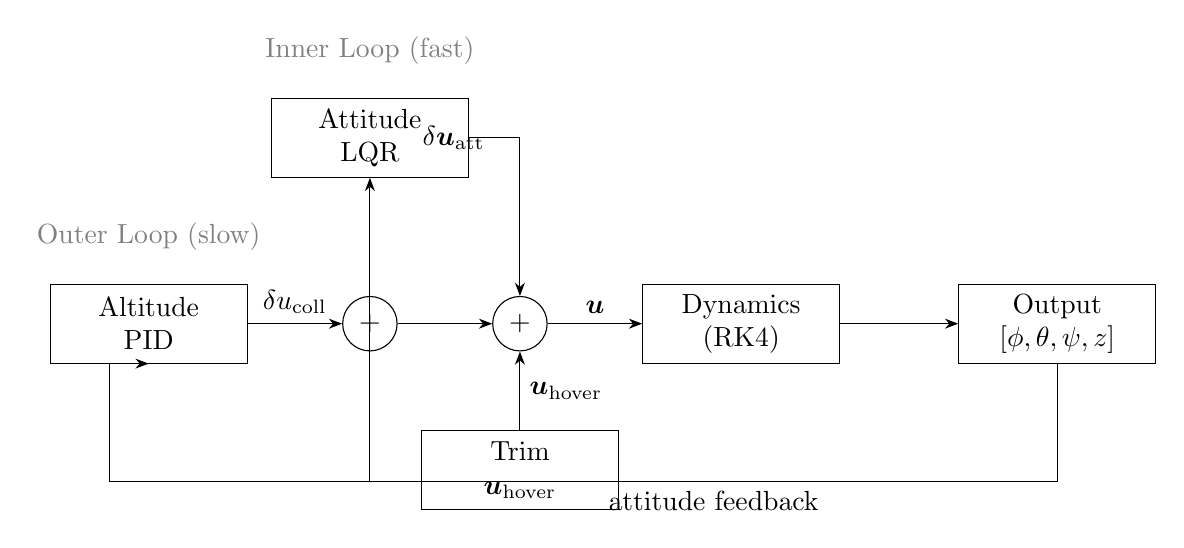
\begin{tikzpicture}[
    block/.style={draw, rectangle, minimum width=2.5cm, minimum height=1cm, align=center},
    sum/.style={draw, circle, minimum size=0.6cm},
    >=Stealth,
    node distance=1.5cm
]
    % Outer loop
    \node[block] (pid) {Altitude\\PID};
    \node[sum, right=1.2cm of pid] (sum1) {$+$};

    % Inner loop
    \node[block, above=1.5cm of sum1] (lqr) {Attitude\\LQR};
    \node[sum, right=1.2cm of sum1] (sum2) {$+$};

    % Plant
    \node[block, right=1.2cm of sum2] (plant) {Dynamics\\(RK4)};

    % Trim
    \node[block, below=1.0cm of sum2] (trim) {Trim\\$\bu_{\text{hover}}$};

    % Clamp
    \node[block, right=1.5cm of plant] (output) {Output\\$[\phi,\theta,\psi,z]$};

    % Connections
    \draw[->] (pid) -- node[above]{$\delta u_{\text{coll}}$} (sum1);
    \draw[->] (lqr) -| node[left, near start]{$\delta \bu_{\text{att}}$} (sum2);
    \draw[->] (sum1) -- (sum2);
    \draw[->] (trim) -- node[right]{$\bu_{\text{hover}}$} (sum2);
    \draw[->] (sum2) -- node[above]{$\bu$} (plant);
    \draw[->] (plant) -- (output);

    % Feedback
    \draw[->] (output.south) -- ++(0,-1.5) -| node[below, near start]{attitude feedback} (lqr.south);
    \draw[->] (output.south) -- ++(0,-1.5) -| node[below, near start]{} ([xshift=-0.5cm]pid.south) -- (pid.south);

    % Labels
    \node[above=0.3cm of lqr, gray] {Inner Loop (fast)};
    \node[above=0.3cm of pid, gray] {Outer Loop (slow)};
\end{tikzpicture}
\caption{Cascaded control architecture.  The inner attitude LQR runs faster (stabilises tilt in $\sim$1 s) while the outer altitude PID runs slower (corrects height over $\sim$3--5 s).}
\end{figure}

% =============================================================================
\section{Software Architecture}
\label{sec:software}
% =============================================================================

\subsection{Project Structure}

\begin{verbatim}
tricopter-lqr/
├── CMakeLists.txt              Build system (CMake)
├── config/
│   └── tricopter_default.yaml  All vehicle and controller parameters
├── include/
│   ├── config.hpp              Configuration structs and loader
│   ├── control_allocation.hpp  B_alloc, B_tau, B_force
│   ├── trim.hpp                Hover trim solver
│   ├── dynamics.hpp            6DOF rigid body dynamics
│   ├── integrator.hpp          RK4 integrator
│   ├── lqr.hpp                 Attitude LQR + CARE solver
│   ├── pid.hpp                 Altitude PID controller
│   └── simulation.hpp          Closed-loop simulation runner
├── src/
│   ├── main.cpp                Entry point
│   ├── config.cpp              YAML parser
│   ├── control_allocation.cpp  Builds B_alloc from rotor config
│   ├── trim.cpp                KKT constrained optimisation
│   ├── dynamics.cpp            State derivative computation
│   ├── integrator.cpp          RK4 step + quaternion renorm
│   ├── lqr.cpp                 CARE solver (matrix sign function)
│   ├── pid.cpp                 PID with anti-windup
│   └── simulation.cpp          Main simulation loop
└── tests/
    └── test_main.cpp           9 unit tests
\end{verbatim}

\subsection{Data Flow}

\begin{enumerate}
    \item \texttt{main.cpp} loads \texttt{tricopter\_default.yaml} into a \texttt{Config} struct.
    \item \texttt{ControlAllocation::build()} constructs $\bB_{\text{alloc}}$, $\bB_\tau$, $\bB_{\text{force}}$.
    \item \texttt{TrimSolver::solve()} finds hover trim $\bu_{\text{hover}}$ via KKT.
    \item \texttt{AttitudeLQR::build()} constructs $\bA$, $\bB$, $\bQ$, $\bR$, solves CARE, computes $\bK$.
    \item \texttt{Simulation::run()} runs the closed-loop sim, writing a CSV log.
\end{enumerate}

\subsection{Build System}

The project uses \textbf{CMake} (version $\geq$ 3.16) with C++17.  Two external libraries are fetched automatically:
\begin{itemize}
    \item \textbf{Eigen3} (v3.4): header-only C++ template library for linear algebra (matrices, vectors, decompositions).
    \item \textbf{yaml-cpp} (v0.8): library for parsing YAML configuration files.
\end{itemize}

Build commands:
\begin{verbatim}
    mkdir build && cd build
    cmake .. -DCMAKE_BUILD_TYPE=Release
    make -j$(nproc)
\end{verbatim}

This produces two executables: \texttt{tricopter\_sim} (main simulation) and \texttt{test\_main} (unit tests).

\subsection{Key Implementation Details}

\subsubsection{Eigen Matrix Types}

Throughout the code, we use Eigen's fixed-size matrices where dimensions are known at compile time:
\begin{lstlisting}[caption={Typical Eigen types used}]
Eigen::Matrix3d          // 3x3 double (rotation, inertia)
Eigen::Vector3d          // 3x1 double (position, angular velocity)
Eigen::Matrix<double,6,6>  // A_att matrix
Eigen::Matrix<double,6,3>  // B_att matrix
Eigen::Matrix<double,3,6>  // K gain matrix
Eigen::VectorXd          // dynamic-size (for variable rotor count)
Eigen::MatrixXd          // dynamic-size matrices
\end{lstlisting}
Fixed-size types are stack-allocated and avoid heap allocation overhead.

\subsubsection{Configuration Loading}

The YAML parser (\texttt{config.cpp}) reads all parameters into C++ structs:
\begin{lstlisting}[caption={Config struct hierarchy}]
struct Config {
    double mass;
    Eigen::Matrix3d J;           // full 3x3 inertia tensor
    std::vector<RotorConfig> rotors;  // variable number of rotors
    AttitudeLQRConfig att_lqr;   // Q_diag, R_diag
    AltitudePIDConfig alt_pid;   // Kp, Ki, Kd, limits
    SimConfig sim;               // dt, duration, perturbation
    double omega_max;            // motor speed limit
};
\end{lstlisting}
The code is parameterised: changing the YAML file (rotor count, geometry, inertia) works without recompilation.

\subsubsection{The Simulation Loop}

Each timestep follows this sequence:
\begin{lstlisting}[caption={Simulation loop pseudocode}]
for step = 0 to num_steps:
    // 1. Extract attitude from quaternion state
    euler = quaternionToEulerZYX(x)
    omega = x[10:13]

    // 2. Build attitude error vector
    delta_x_att = [euler; omega]  // desired = zero

    // 3. Inner loop: attitude LQR
    delta_u_att = -K * delta_x_att

    // 4. Outer loop: altitude PID
    z_err = z_desired - x[2]
    pid_out = pid.update(z_err, x[2], dt)
    T_cmd = m*g + pid_out
    delta_u_coll = (T_cmd - T_hover) / (N * k_T_avg)

    // 5. Combine and clamp
    u = u_hover + delta_u_att + delta_u_coll
    u = clamp(u, 0, omega_max^2)

    // 6. Integrate with RK4
    x = rk4Step(dynamics, x, u, dt)

    // 7. Log to CSV
\end{lstlisting}

% =============================================================================
\section{Unit Tests}
\label{sec:tests}
% =============================================================================

We have 9 unit tests that verify correctness:

\begin{table}[H]
\centering
\small
\begin{tabular}{lp{8cm}}
\toprule
\textbf{Test} & \textbf{What it checks} \\
\midrule
\texttt{balloc\_dimensions} & $\bB_{\text{alloc}}$ is $6 \times N$, $\bB_\tau$ is $3 \times N$, $\bB_{\text{force}}$ is $3 \times N$. \\
\texttt{balloc\_force\_values} & Each force column equals $k_T \cdot [0,0,1]^T$ (hand-computed). \\
\texttt{balloc\_torque\_values} & Torque columns match the cross-product + drag formula (hand-computed). \\
\texttt{trim\_residual\_torque} & Residual torque is finite and bounded ($< 1$ Nm). \\
\texttt{trim\_thrust\_balance} & Total hover thrust $= mg$ within 0.01 N. \\
\texttt{care\_p\_spd} & CARE solution $\bP$ is symmetric and all eigenvalues $> 0$ (positive definite). \\
\texttt{care\_closed\_loop} & All 6 eigenvalues of $(\bA - \bB\bK)$ have $\text{Re}(\lambda) < 0$ (closed-loop stable). \\
\texttt{quat\_normalisation} & After 100 RK4 steps, $\|\bq\| = 1.0 \pm 10^{-10}$. \\
\texttt{pid\_step\_response} & PID converges a simple double-integrator to setpoint within 10\% in 10 s. \\
\bottomrule
\end{tabular}
\caption{Unit test descriptions.  All 9 tests pass.}
\end{table}

% =============================================================================
\section{Simulation Results}
\label{sec:results}
% =============================================================================

\subsection{Simulation Parameters}

\begin{itemize}
    \item Timestep: $\Delta t = 0.001$ s (1 kHz)
    \item Duration: 10 s
    \item Initial perturbation: 5° roll, 3° pitch, 0° yaw
    \item Impulse disturbance at $t = 2$ s: $[0.1, 0.05, 0.02]$ Nm for 10 ms
    \item Desired altitude: $z = 0$ (hover at origin)
\end{itemize}

\subsection{Key Observations}

\begin{enumerate}
    \item \textbf{Roll and pitch} remain bounded within $\pm 15°$ throughout the simulation, demonstrating effective attitude regulation.

    \item \textbf{Yaw drifts continuously}, cycling through $360°$ repeatedly.  This is the expected consequence of the 0.091 Nm residual yaw torque from the trim.  The LQR's yaw channel (eigenvalues at $-0.095 \pm 0.095j$, time constant $\approx 10.5$ s) is too slow to fully reject this constant disturbance.

    \item \textbf{Altitude decreases} because the yaw drift tilts the thrust vector sideways, reducing the vertical component of thrust.  The altitude PID cannot compensate fast enough.

    \item The \textbf{torque disturbance at $t = 2$ s} causes a brief spike in roll/pitch that is damped within $\sim 2$ s, showing good disturbance rejection.
\end{enumerate}

\subsection{The Under-Actuation Problem}

The yaw drift is \textbf{not} a controller bug --- it is a fundamental \emph{physical} limitation.  With analysis:
\begin{itemize}
    \item Roll balance requires $u_2 = u_3$ (due to symmetric $y$-positions of rear rotors).
    \item Pitch balance requires $u_1 = 1.2 \, u_3$ (due to arm length ratio $0.25/0.15 = 5/3$).
    \item Yaw balance with $[+1, -1, +1]$ spin directions requires $u_1 - u_2 + u_3 = 0$.
    \item Substituting: $1.2 u_3 - u_3 + u_3 = 1.2 u_3 \neq 0$.
\end{itemize}

No choice of spin directions $d_i \in \{+1, -1\}$ can satisfy $1.2 d_1 + d_2 + d_3 = 0$ because $1.2$ is not an integer.  The vehicle fundamentally cannot hover without yaw drift unless the geometry is changed (e.g., symmetric arm lengths) or a yaw servo is added.

% =============================================================================
\section{Hardware Considerations}
\label{sec:hardware}
% =============================================================================

\subsection{What Happens at the Hardware Level}

While our code runs as a simulation, the same algorithms would execute on a real flight controller.  Here is how each software component maps to hardware:

\subsubsection{Sensors (Input)}
\begin{itemize}
    \item \textbf{IMU (Inertial Measurement Unit):} A MEMS chip (e.g., MPU-6050) provides 3-axis accelerometer and 3-axis gyroscope readings at $\sim$1 kHz.  The gyroscope gives $\bomega$ directly.  The accelerometer is fused with the gyroscope via a complementary filter or extended Kalman filter to estimate the quaternion $\bq$.
    \item \textbf{Barometer:} Provides altitude $z$ at $\sim$100 Hz.  Some designs also use a downward-facing ultrasonic or lidar sensor for more accurate altitude hold.
\end{itemize}

\subsubsection{Computation (Processing)}
\begin{itemize}
    \item The LQR gain $\bK$ is computed \textbf{offline} (once, at startup).  The matrix sign function iteration takes $\sim$10 ms on a modern CPU.  On a flight controller MCU (e.g., STM32F4), this could take $\sim$100 ms but only needs to run once.
    \item At runtime, the control law $\delta\bu = -\bK \cdot \delta\bx$ is a single matrix-vector multiply: 3 rows $\times$ 6 columns $=$ 18 multiply-add operations.  This takes $< 1\,\mu$s even on a 168 MHz ARM Cortex-M4.
    \item The PID is similarly trivial: $\sim$10 floating-point operations per timestep.
    \item The RK4 integrator is \emph{not} needed on real hardware --- the real physics \emph{is} the integrator.  RK4 is only for simulation.
\end{itemize}

\subsubsection{Actuators (Output)}
\begin{itemize}
    \item The control output $u_i = \omega_i^2$ must be converted to a motor command.  Brushless DC motors are driven by \textbf{Electronic Speed Controllers (ESCs)} that accept a PWM (pulse-width modulation) signal.
    \item The mapping from $\omega^2$ to PWM duty cycle is typically linearised through a motor test: spin the motor at known PWM values, measure $\omega$ with a tachometer, and fit a polynomial.
    \item The clamping $u_i \in [0, \omega_{\max}^2]$ prevents requesting speeds beyond the motor's capability.
\end{itemize}

\subsection{Timing Requirements}

The inner attitude loop must run at $\geq$ 250 Hz (ideally 1 kHz) because rotational dynamics are fast.  The outer altitude loop can run at $\sim$50--100 Hz because vertical dynamics are slower.  In our simulation, both loops run at 1 kHz for simplicity.

\subsection{Real-World Differences}

In a real implementation, additional considerations include:
\begin{itemize}
    \item \textbf{Sensor noise:} Low-pass filtering on gyroscope data, complementary filter for attitude estimation.
    \item \textbf{Motor dynamics:} Brushless motors have a time constant ($\sim$20--50 ms) that delays the response.  The LQR model assumes instantaneous motor response.
    \item \textbf{Propeller flex and vibration:} High-frequency vibrations from the propellers can corrupt accelerometer readings.
    \item \textbf{Battery voltage sag:} As the battery discharges, the same PWM signal produces less thrust.  A voltage compensation factor is needed.
\end{itemize}

% =============================================================================
\section{Mathematical Summary}
\label{sec:math_summary}
% =============================================================================

For quick reference, here are all the key equations in order:

\begin{enumerate}
    \item \textbf{Thrust and drag:} $T_i = k_T \omega_i^2$, \; $Q_i = k_Q \omega_i^2$

    \item \textbf{Allocation:} $[\bF; \btau] = \bB_{\text{alloc}} \bu$

    \item \textbf{Torque per rotor:} $\btau_i = \bm{r}_i \times (k_T \hat{\bm{t}}_i) + d_i k_Q \hat{\bm{s}}_i$ \; (per unit $\omega_i^2$)

    \item \textbf{Trim (KKT):}
    $\begin{bmatrix} 2\bm{M} & \bm{c} \\ \bm{c}^T & 0 \end{bmatrix}
    \begin{bmatrix} \bu \\ \lambda \end{bmatrix}
    = \begin{bmatrix} \bm{0} \\ mg \end{bmatrix}$
    where $\bm{M} = \bB_\tau^T \bB_\tau$

    \item \textbf{Translational dynamics:} $m\dot{\bm{v}} = \bm{R}(\bq) \bF_{\text{body}} + m\bm{g}$

    \item \textbf{Rotational dynamics:} $\bJ\dot{\bomega} = \btau - \bomega \times (\bJ\bomega)$

    \item \textbf{Quaternion kinematics:} $\dot{\bq} = \frac{1}{2}\bq \otimes [0; \bomega]$

    \item \textbf{RK4:} $\bx_{k+1} = \bx_k + \frac{\Delta t}{6}(\bm{k}_1 + 2\bm{k}_2 + 2\bm{k}_3 + \bm{k}_4)$

    \item \textbf{Linearised attitude:} $\delta\dot{\bx} = \bA\delta\bx + \bB\delta\bu$ where $\bA = \begin{bsmallmatrix} \bzero & \bI \\ \bzero & \bzero \end{bsmallmatrix}$, $\bB = \begin{bsmallmatrix} \bzero \\ \bJ^{-1}\bB_\tau \end{bsmallmatrix}$

    \item \textbf{CARE:} $\bA^T\bP + \bP\bA - \bP\bB\bR^{-1}\bB^T\bP + \bQ = \bzero$

    \item \textbf{LQR gain:} $\bK = \bR^{-1}\bB^T\bP$

    \item \textbf{Control law:} $\bu = \bu_{\text{hover}} - \bK\delta\bx_{\text{att}} + \delta u_{\text{coll}} \cdot \bm{1}$
\end{enumerate}

% =============================================================================
\section{Conclusion}
% =============================================================================

We have built a complete flight controller for a servoless asymmetric tricopter from first principles.  The cascaded architecture (inner attitude LQR + outer altitude PID) successfully separates the fast rotational dynamics from the slower translational dynamics.

The CARE equation was solved using the matrix sign function applied to the Hamiltonian --- a numerically robust method that handles the poorly conditioned system arising from the small $\bB$ matrix entries.

The simulation revealed a fundamental limitation: a servoless tricopter with this rotor geometry and spin directions $[+1, -1, +1]$ \emph{cannot} achieve torque-free hover.  The residual yaw torque of 0.091 Nm causes continuous yaw drift.  This is not a controller deficiency but a physical under-actuation: 3 actuators cannot independently control 3 torques plus thrust (4 constraints).  The solution requires either a yaw servo (4th actuator), tilted rotor axes, or a modified rotor geometry where the arm lengths form integer ratios with the spin direction assignment.

Despite this limitation, the controller demonstrates:
\begin{itemize}
    \item Bounded roll and pitch errors ($\pm 15°$) from a $5°/3°$ initial perturbation.
    \item Effective impulse disturbance rejection within $\sim$2 seconds.
    \item All closed-loop eigenvalues with negative real parts (provably stable linearised system).
    \item CARE residual of $2.4 \times 10^{-11}$ (machine-precision accuracy).
    \item All 9 unit tests passing.
\end{itemize}

\end{document}
